\documentclass[14pt]{extarticle}
\usepackage[english,ukrainian]{babel}
\usepackage[utf8]{inputenc}
\usepackage{amsmath,amssymb}
\usepackage{parskip}
\usepackage{graphicx}
\usepackage{xcolor}
\usepackage{tcolorbox}
\tcbuselibrary{skins}
\usepackage[framemethod=tikz]{mdframed}
\usepackage{chngcntr}
\usepackage{enumitem}
\usepackage{hyperref}
\usepackage{float}
\usepackage{subfig}
\usepackage{esint}
\usepackage[top=2.5cm, left=3cm, right=3cm, bottom=4.0cm]{geometry}
\usepackage[table]{xcolor}
\usepackage{algorithm}
\usepackage{algpseudocode}
\usepackage{listings}
\usepackage{dsfont}

\usepackage{tikz}

\tcbuselibrary{theorems}

\newtcbtheorem[number within=section]{statement}{Твердження}%
{colback=blue!5,colframe=blue!35!black,fonttitle=\bfseries}{th}

\newtcbtheorem[number within=section]{theorem}{Теорема}%
{colback=green!5,colframe=green!35!black,fonttitle=\bfseries}{th}

\newtcbtheorem[number within=section]{def}{Означення}%
{colback=red!5,colframe=red!35!black,fonttitle=\bfseries}{th}

\newtcbtheorem[number within=section]{example}{Приклад}%
{colback=yellow!5,colframe=yellow!35!black,fonttitle=\bfseries}{th}

\def\f[#1]{sin(3*#1)/2+#1/3+1}
\def\Tick(#1)#2{%
    \rput[b](#1|0,-12pt){\small$#2$}
    \psline(#1|0,0)(#1|0,-2pt)
}

\title{Екзаменаційна робота з навчальної дисципліни ``Чисельний аналіз''}
\author{Студента 3 курсу групи МП-31 Захарова Дмитра Олеговича}
\date{\today}

\begin{document}

\maketitle

\begin{center}
    \textbf{Білет \#3}
\end{center}
\section*{Питання 1.}

\textbf{Умова.} Обчислити інтеграл за формулою трапецій і оцінити похибку обчислення:
\[
\mathcal{I} = \int_{[0,1]} \cos x^2 dx, \; n = 5
\]
\textbf{Розв'язок.} Будемо вважати, що $n=5$ відповідає розбиттю інтервалу на $n$ частин (тобто, маємо $n+1$ вузлів). 

Отже, маємо інтервал $[0,1]$. Розбиваємо його рівномірно, тоді маємо вузли:
\[
x_k = \frac{k}{5}, \; k \in \{0,\dots,5\}, \; h = \frac{1}{5}
\]
Згадаємо з теорії, що квадратурна формула трапеції має вигляд:
\[
\int_{[\alpha,\beta]} f(x)dx \approx \frac{(\beta-\alpha)(f(\alpha)+f(\beta))}{2}
\]
Проте, застосування цієї формули безпосередньо на всьому відрізку $[0,1]$ не дасть точного результату, тому скористаємося складеною квадратурною формулу трапеції:
\begin{gather*}
\mathcal{I}_1 = \int_{[0,1]}\cos x^2 dx \approx \sum_{k=1}^5 \int_{[x_{k-1},x_k]}\cos x^2 dx \\
= \sum_{k=1}^5 \frac{1}{10}\left(\cos \left(\frac{k-1}{5}\right)^2 + \cos\left(\frac{k^2}{25}\right)\right)
\end{gather*}
Далі залишається акуратно порахувати цей вираз. Маємо:
\begin{gather*}
\mathcal{I}_1 = \frac{1}{10}\Big(\cos 0 + \cos \frac{1}{25} + \cos \frac{1}{25} + \cos \frac{4}{25} + \cos \frac{4}{25} \\ + \cos \frac{9}{25}+\cos \frac{9}{25} + \cos \frac{16}{25}+\cos \frac{16}{25} + \cos 1\Big) \approx 0.8989
\end{gather*}

Візуально, процес знаходження цього інтегралу зображено на рис. \ref{fig:1}. 

\begin{figure}[H]
    \centering
    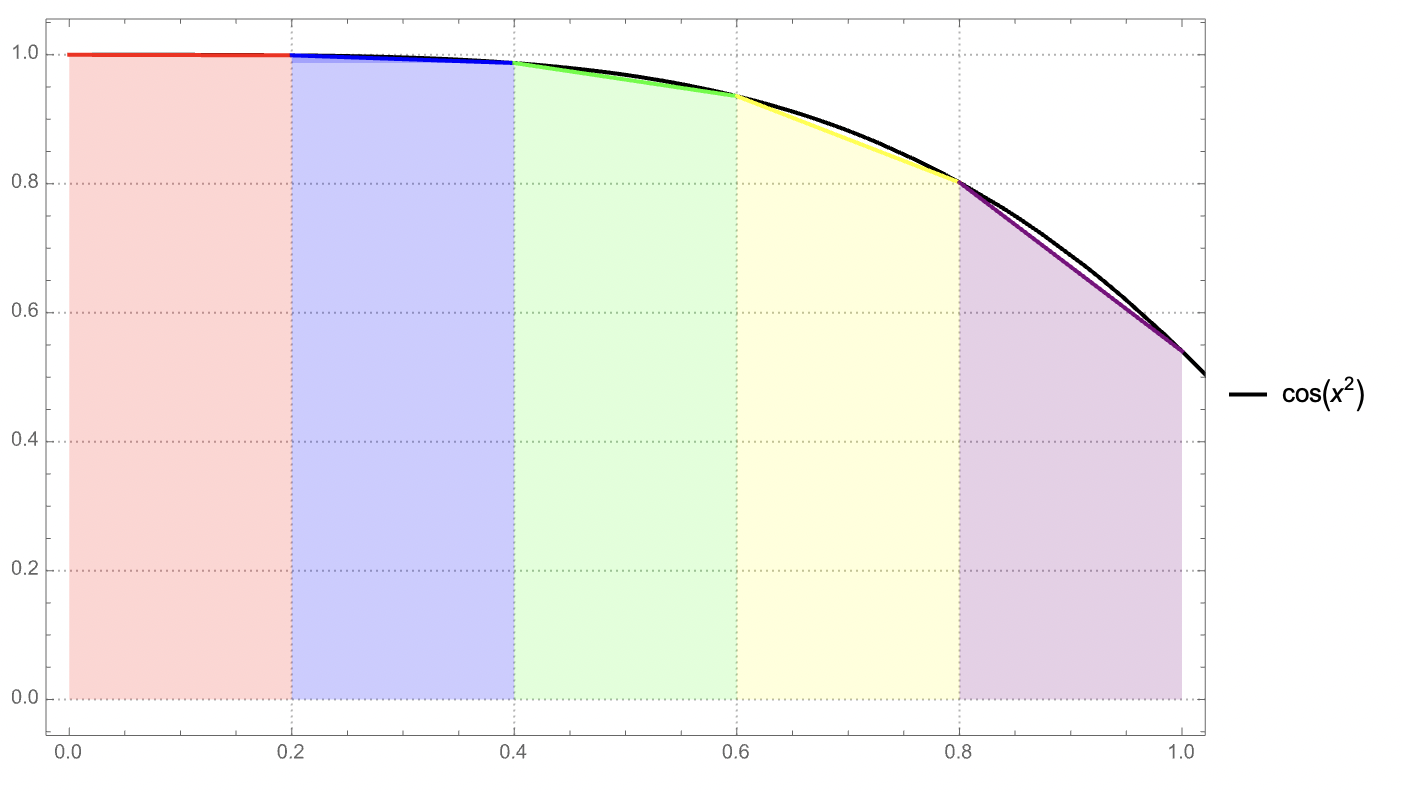
\includegraphics[width=\textwidth]{images/exam/plot.png}
    \caption{Знаходження інтегралу методом трапецій}
    \label{fig:1}
\end{figure}

Таким чином, значення нашого інтегралу $\mathcal{I} \approx \mathcal{I}_1 \approx 0.8989$. Тепер оцінимо похибку $\Delta := |\mathcal{I} - \mathcal{I}_1|$:
\[
\Delta \leq \frac{\mu_2(\beta-\alpha)h^2}{12} = \frac{1}{25 \cdot 12} \max_{x \in [0,1]}|(\cos x^2)''|
\]
Тепер треба оцінити $\max_{x \in [0,1]}|(\cos x^2)''|$. Знайдемо другу похідну:
\[
|(\cos x^2)''| = |(2x \sin x^2)'| = |2\sin x^2 + 4x^2 \cos x^2|
\]
Оцінимо цей вираз наступним чином:
\[
\max_{x \in [0,1]}|2\sin x^2 + 4x^2\cos x^2| \leq 6
\]
В такому разі похибка:
\[
\Delta \leq \frac{6}{25 \cdot 12} = \frac{1}{50}
\]
\textbf{Відповідь.} $\mathcal{I}_1 \approx 0.8989, \; |\mathcal{I}-\mathcal{I}_1| \leq 0.02$. 

\end{document}

